\documentclass[10pt]{article}
\usepackage{tikz}
\usetikzlibrary{shapes.misc}
\usepackage[margin=0cm]{geometry}
\pagestyle{empty}
\tikzstyle{every node}=[cross out, draw, red]

\begin{document}

\vspace*{\fill}
\begin{center}
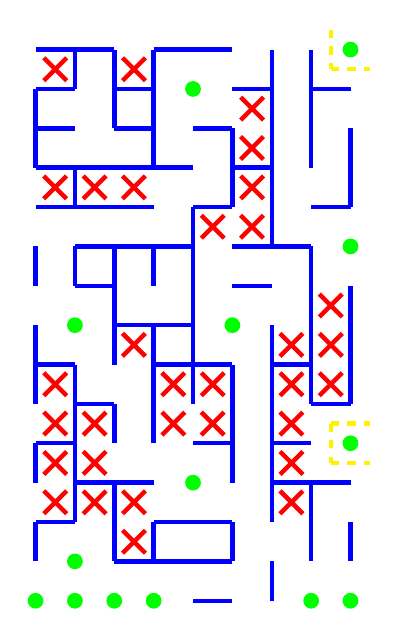
\begin{tikzpicture}[x=0.5cm, y=-0.5cm, ultra thick, blue]
% Walls
    \draw (0,0) -- (2,0);
    \draw (3,0) -- (5,0);
    \draw (0,1) -- (1,1);
    \draw (2,1) -- (3,1);
    \draw (5,1) -- (6,1);
    \draw (7,1) -- (8,1);
    \draw (0,2) -- (1,2);
    \draw (2,2) -- (3,2);
    \draw (4,2) -- (5,2);
    \draw (0,3) -- (4,3);
    \draw (5,3) -- (6,3);
    \draw (0,4) -- (3,4);
    \draw (4,4) -- (5,4);
    \draw (7,4) -- (8,4);
    \draw (1,5) -- (4,5);
    \draw (5,5) -- (7,5);
    \draw (1,6) -- (2,6);
    \draw (5,6) -- (6,6);
    \draw (2,7) -- (4,7);
    \draw (0,8) -- (1,8);
    \draw (3,8) -- (5,8);
    \draw (6,8) -- (7,8);
    \draw (1,9) -- (2,9);
    \draw (7,9) -- (8,9);
    \draw (0,10) -- (1,10);
    \draw (4,10) -- (5,10);
    \draw (6,10) -- (7,10);
    \draw (1,11) -- (3,11);
    \draw (6,11) -- (8,11);
    \draw (0,12) -- (1,12);
    \draw (3,12) -- (5,12);
    \draw (2,13) -- (5,13);
    \draw (4,14) -- (5,14);
    \draw (0,1) -- (0,3);
    \draw (0,5) -- (0,6);
    \draw (0,7) -- (0,9);
    \draw (0,10) -- (0,11);
    \draw (0,12) -- (0,13);
    \draw (1,0) -- (1,1);
    \draw (1,3) -- (1,4);
    \draw (1,5) -- (1,6);
    \draw (1,8) -- (1,12);
    \draw (2,0) -- (2,2);
    \draw (2,5) -- (2,8);
    \draw (2,9) -- (2,10);
    \draw (2,11) -- (2,13);
    \draw (3,0) -- (3,3);
    \draw (3,5) -- (3,6);
    \draw (3,7) -- (3,10);
    \draw (3,12) -- (3,13);
    \draw (4,4) -- (4,9);
    \draw (5,2) -- (5,4);
    \draw (5,8) -- (5,11);
    \draw (5,12) -- (5,13);
    \draw (6,0) -- (6,5);
    \draw (6,7) -- (6,12);
    \draw (6,13) -- (6,14);
    \draw (7,0) -- (7,3);
    \draw (7,5) -- (7,9);
    \draw (7,11) -- (7,13);
    \draw (8,2) -- (8,4);
    \draw (8,6) -- (8,9);
    \draw (8,12) -- (8,13);
% Pillars
    \fill[green] (8,0) circle(0.2);
    \fill[green] (4,1) circle(0.2);
    \fill[green] (8,5) circle(0.2);
    \fill[green] (1,7) circle(0.2);
    \fill[green] (5,7) circle(0.2);
    \fill[green] (8,10) circle(0.2);
    \fill[green] (4,11) circle(0.2);
    \fill[green] (1,13) circle(0.2);
    \fill[green] (0,14) circle(0.2);
    \fill[green] (1,14) circle(0.2);
    \fill[green] (2,14) circle(0.2);
    \fill[green] (3,14) circle(0.2);
    \fill[green] (7,14) circle(0.2);
    \fill[green] (8,14) circle(0.2);
% Inner points in accessible cul-de-sacs
    \node at (0.5,0.5) {};
    \node at (2.5,0.5) {};
    \node at (5.5,1.5) {};
    \node at (5.5,2.5) {};
    \node at (0.5,3.5) {};
    \node at (1.5,3.5) {};
    \node at (2.5,3.5) {};
    \node at (5.5,3.5) {};
    \node at (4.5,4.5) {};
    \node at (5.5,4.5) {};
    \node at (7.5,6.5) {};
    \node at (2.5,7.5) {};
    \node at (6.5,7.5) {};
    \node at (7.5,7.5) {};
    \node at (0.5,8.5) {};
    \node at (3.5,8.5) {};
    \node at (4.5,8.5) {};
    \node at (6.5,8.5) {};
    \node at (7.5,8.5) {};
    \node at (0.5,9.5) {};
    \node at (1.5,9.5) {};
    \node at (3.5,9.5) {};
    \node at (4.5,9.5) {};
    \node at (6.5,9.5) {};
    \node at (0.5,10.5) {};
    \node at (1.5,10.5) {};
    \node at (6.5,10.5) {};
    \node at (0.5,11.5) {};
    \node at (1.5,11.5) {};
    \node at (2.5,11.5) {};
    \node at (6.5,11.5) {};
    \node at (2.5,12.5) {};
% Entry-exit paths without intersections
    \draw[dashed, yellow] (7.5,0.5) -- (8.5,0.5);
    \draw[dashed, yellow] (7.5,9.5) -- (8.5,9.5);
    \draw[dashed, yellow] (7.5,10.5) -- (8.5,10.5);
    \draw[dashed, yellow] (7.5,-0.5) -- (7.5,0.5);
    \draw[dashed, yellow] (7.5,9.5) -- (7.5,10.5);
\end{tikzpicture}
\end{center}
\vspace*{\fill}

\end{document}
